
%--------------------------------------------------------------------
%--------------------------------------------------------------------
% Formato para los talleres del curso de Herramientas Computacionales
% Universidad de los Andes
% 2015-10
%--------------------------------------------------------------------
%--------------------------------------------------------------------

\documentclass[11pt,letterpaper]{exam}
\usepackage[utf8]{inputenc}
\usepackage[spanish]{babel}
\usepackage{graphicx}
%\usepackage{mdframed}
%\usepackage{tabularx}
\usepackage[absolute]{textpos} % Para poner una imagen completa en la portada
%\usepackage{multirow}
%\mdfdefinestyle{mystyle}{leftmargin=1cm,rightmargin=1cm,linecolor=red}
%\usepackage{float}
%\usepackage{hyperref}
\decimalpoint


\newcommand{\base}[1]{\underline{\hspace{#1}}}
\boxedpoints
\pointname{ pt}
%\extrawidth{0.75in}
%\extrafootheight{-0.5in}
\extraheadheight{-0.15in}
%\pagestyle{head}

%\noprintanswers
%\printanswers
\renewcommand{\solutiontitle}{}
\SolutionEmphasis{\color{blue}}

\usepackage{upquote,textcomp}
\newcommand\upquote[1]{\textquotesingle#1\textquotesingle} % To fix straight quotes in verbatim

\begin{document}
\begin{center}
{\Large Herramientas Computacionales} \\
Taller 5 - \textsc{Python 2}:\\
%Definición de funciones, tipos de variables y \\ recursividad. \\
Fecha de publicación: {\small \it marzo de 2015}\\
\end{center}

\begin{textblock*}{40mm}(10mm,20mm)
  
\includegraphics[width=3cm]{logoUniandes.png}
\end{textblock*}

\begin{textblock*}{40mm}(161mm,20mm)
  
\includegraphics[width=3cm]{logoUniandes.png}
\end{textblock*}

\vspace{0.5cm}

\noindent Este taller debe hacerse en grupos de 2 personas.\\
El código que de solución a este taller debe ser entregado en un solo archivo con nombre:\\
 \verb+ApellidoEstudiante1-ApellidoEstudiante2_HW5.py o .ipynb+ a través de \textbf{Sicuaplus}.\\

En cada parte del ejercicio se entrega 1/3  de los puntos si el código propuesto es razonable, 1/3 si se puede ejecutar y 1/3 si entrega resultados correctos. El código debe llevar comentarios suficientes.

\vspace{0.5cm}

\begin{questions}

\question[100] {\bf Blackjack:}
Escriba un programa en \verb+Python+ donde un usuario juegue blackjack con el computador. La baraja usada debe tener 52 cartas. En su código haga corresponder números a las diferentes cartas de acuerdo al siguiente esquema: 1 $\rightarrow$ Az, 2-10 $\rightarrow$ 2-10, 11 $\rightarrow$ J, 12 $\rightarrow$ Q, 13 $\rightarrow$ K. La baraja sin barajar correspondería a la siguiente lista: 

$[ 1,2,3,4,5,6,7,8,9,10,11,12,13,$
$1,2,3,4,5,6,7,8,9,10,11,12,13,$
$1,2,3,4,5,6,7,8,9,10,11,12,13,$
$1,2,3,4,5,6,7,8,9,10,11,12,13]$

\begin{parts}
	\part[40] El programa debe tener al menos 5 funciones que hagan lo siguiente.\\
	\begin{subparts}
		%\subpart[6]  leer las cartas de \verb+cartas.txt+,
		\subpart[6] Barajar las cartas de la baraja.
		\subpart[6] Recibir las cartas de un jugador e imprimirlas.
		\subpart[8] Tomar la primera carta de la baraja, entregarla y retirarla del mismo.
		\subpart[10] Recibir un conjunto de cartas y calcular el mayor total menor o igual a 21, o en su defecto el menor total.
		\subpart[10] Recibir los totales del jugador y el computador y decidir el ganador.
	\end{subparts}
\vspace{0.2cm}

\part[40]

En el programa el computador debe jugar automáticamente pidiendo más cartas siempre que su total sea menor a 17. Al terminar el programa debe decidir quien de los dos ha ganado.

\part[20] El programa debe ser interactivo y debe ser clara la forma de jugar.
\begin{itemize}
\item Se debe preguntar al jugador si desea más cartas (use \verb+raw_input+):
\item Se deben imprimir las cartas del jugador y del computador.
\end{itemize}


\end{parts}
\vspace{1cm}
{\bf Ayudas y Bono:} 

\begin{itemize}

\item Para barajar aleatoriamente escoja una posición al azar entre 0 y N-1 de la lista en donde están las cartas.
      Intercambie los elementos de la posición $0$ y de la posición aleatoria.  Luego escoja una posición al azar
      entre $1$ y $N-1$ e intercambie los elementos de la posición $1$ y la posición aleatoria. Así sucesivamente hasta que halla barajado todo la baraja.
\item Para sumar recuerde que el ``Az'' puede valer 1 o 11 y que cada figura (J, Q o K) vale 10.
\item Cada vez que un usuario pida una carta el código debe imprimir las cartas de cada jugador. 
\item Bono de 15 puntos: escriba una función que imprima las cartas con algún diseño gráfico.

\end{itemize}

\end{questions}


\begin{figure}[h!]
\begin{center}
	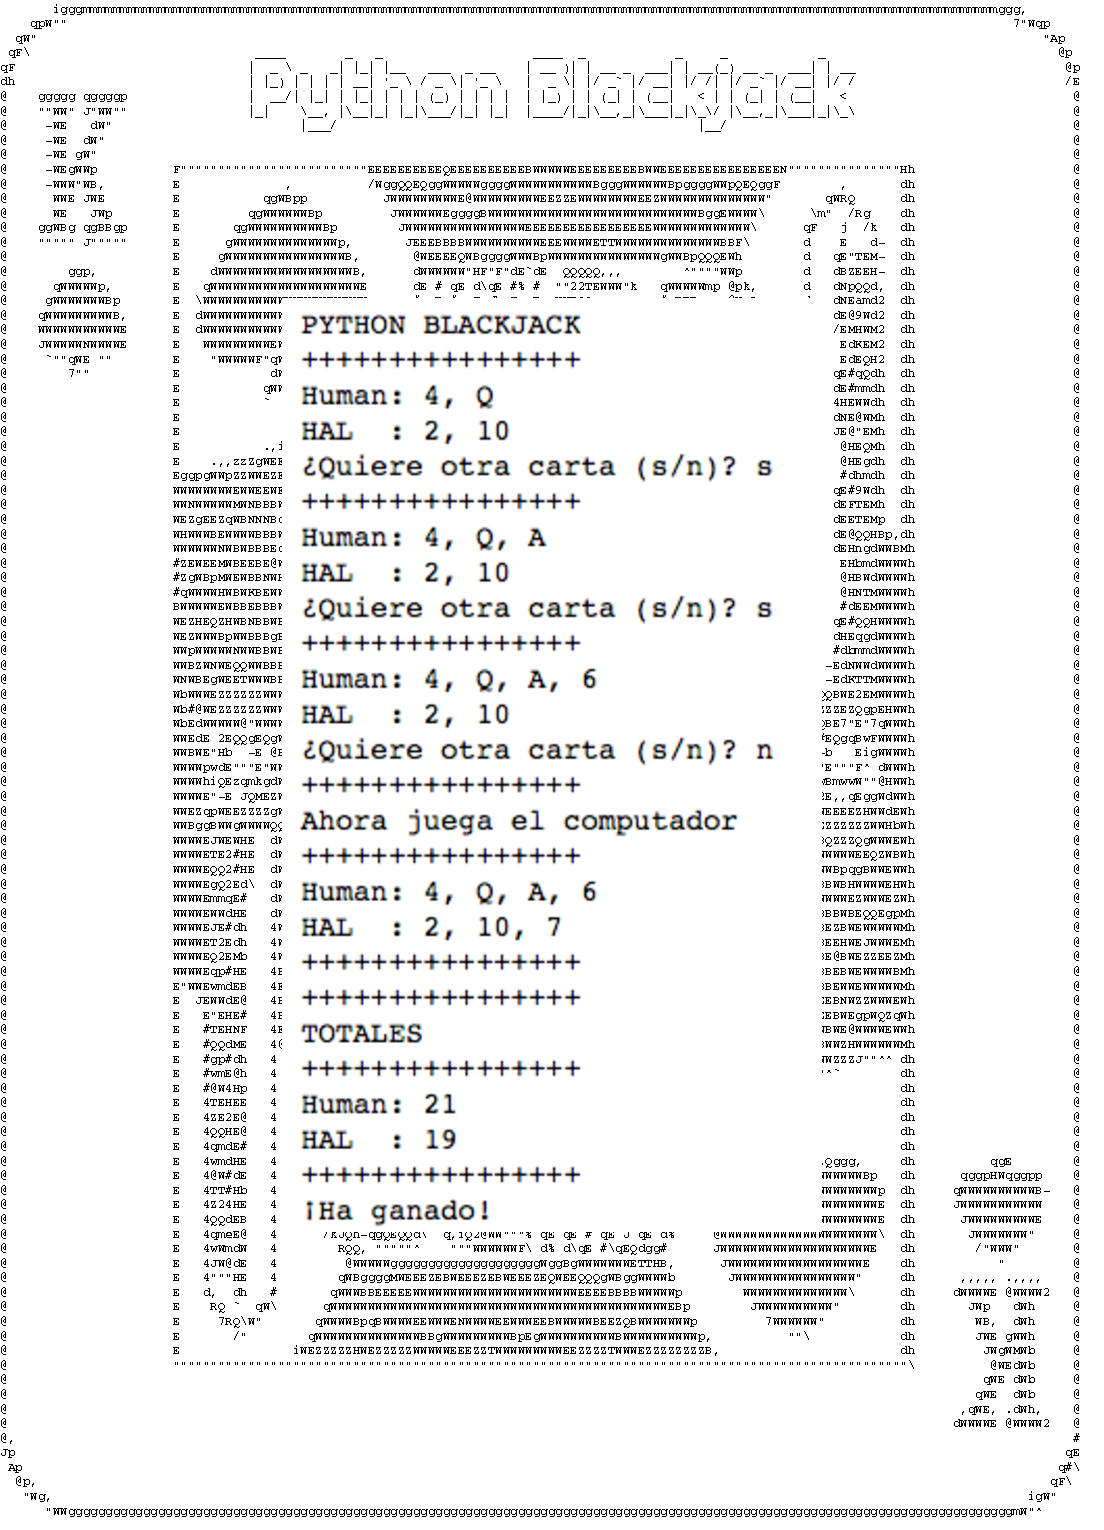
\includegraphics[width=0.8\textwidth]{./pyblackj.pdf}
\end{center}
\end{figure}
%\newpage
%\newpage
%
%\[
%R(\pi/2)=\left(\begin{tabular}{cc}
% $\frac{1}{\sqrt{2}}$ & $-\frac{1}{\sqrt{2}}$ \\
% $\frac{1}{\sqrt{2}}$ & $\frac{1}{\sqrt{2}}$ 
%\end{tabular}\right)
%\]
%
%\newpage
%
%\begin{center}
%{\it Humpty Dumpty sat on a wall,}\\
%{\bf Humpty Dumpty had a great fall.}\\
%\underline{All the king's horses and all the king's men}\\
%Couldn't put Humpty together again.
%\end{center}

\end{document}
